\section{Overdetermined systems}

\begin{definition}[\textit{Overdetermined system}]
    A linear system $Ax=b$ with $A \in \mathbb{R}^{m \times n}$ is called overdetermined if $m>n$. 
\end{definition}
\begin{definition}[\textit{Underdetermined system}]
    A linear system $Ax=b$ with $A \in \mathbb{R}^{m \times n}$ is called underdetermined if $m<n$. 
\end{definition}

An overdetermined system $Ax=b$ generally has no solution unless the vector $b$ is an element of range($A$), where: 
\[\textnormal{range}(A)=\{z \in \mathbb{R}^n|z=Ay \textnormal{ for } y \in \mathbb{R}^n\}\]
In general, for an arbitrary $b$ we can search for a vector $x \in \mathbb{R}^n$ that minimizes the Euclidean norm of the residual, that is: 
\[x=\argmin_{y \in \mathbb{R}^n}\left( \dfrac{1}{2}\left\lVert r(y) \right\rVert^2 \right)=\dfrac{1}{2}\left\lVert b-Ay \right\rVert^2 = \Phi (y)\]
To find the minimum of the argument we have to choose an $x$ such that $\nabla\Phi(x)=0$. 
By expanding the previous formula we have that: 
\[\Phi(y)=\dfrac{1}{2}\left( b-Ay \right)^T\left( b-Ay \right)=\dfrac{1}{2}\left( \left\lVert b \right\rVert^2 -b^TAy-y^TA^Tb+y^TA^TAy\right)=\dfrac{1}{2}\left( \left\lVert b \right\rVert^2-2y^TA^Tb+y^TA^TAy\right)\]
We can now derive the previous formula, obtaining: 
\[\Phi^{'}(y)=A^Tb-A^TAy\]
To find the minimum we set the derivative equal zero obtaining that: 
\[A^TAx=A^Tb\]
If $A$ is full rank with $m \geq n$, then $A^TA$ is non-singular. 

\paragraph*{QR factorization}
A matrix $A \in \mathbb{R}^{m \times n}$ and full rank admits a unique factorization: 
\[A=QR\]
Here, $Q \in \mathbb{R}^{m \times m}$ is an orthogonal matrix (i.e., $Q^TQ=I$), while $R \in \mathbb{R}^{m \times n}$ is an upper trinagular matrix
\begin{figure}[H]
    \centering
    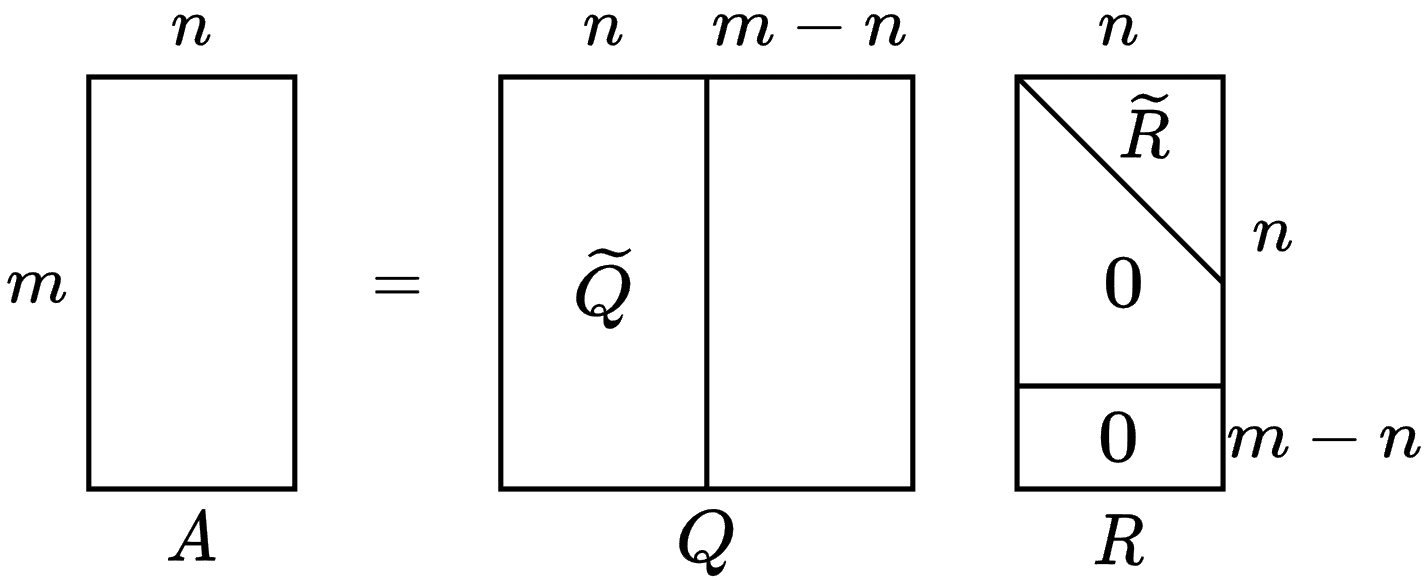
\includegraphics[width=0.5\linewidth]{images/qr.png}
    \caption{The QR factorization}
\end{figure}
We now substitute in the formula the factorization, obtaining: 
\[Q^TR^TQRx=Q^TR^Tb\]
By definition, $Q^TQ=I$: 
\[R^TRx=A^Tb\]
That can be solved with a backward ($Rx=y$) and a forward ($R^Ty=A^Tb$) substitution. 
If we use the slim matrices $\widetilde{Q}$ and $\widetilde{R}$ we will have: 
\[\widetilde{R}^T\widetilde{Q}^T\widetilde{Q}\widetilde{R}x=\widetilde{R}^T\widetilde{Q}^Tb\]
That is: 
\[\widetilde{R}x=\widetilde{Q}^Tb\]
That can be simply solved with a backwardf substitution. 

\paragraph*{Singular value factorization}
Let $A \in \mathbb{R}^{m \times n}$ with rank $r \leq \min(m,n)$. 
There existst a factorization of the form: 
\[A=U\Sigma V^T\]
Here, $U \in \mathbb{R}^{m \times m}$ orthogonal matrix, $V \in \mathbb{R}^{n \times n}$ orthogonal matrix, and $\Sigma \in \mathbb{R}^{m \times n}=\text{diag}(\sigma_1,\dots,\sigma_p)$, where $p=\min(m,n)$ and $\sigma_1 \geq \dots \geq \sigma_p \geq 0$. 
The $\sigma_i$ are celled singular values and are the quare root of the eigenvalues of $A^TA$. 

\paragraph*{Least square}
Let's consider $Ax=b$ for $A \in \mathbb{R}^{m \times n}$. 
We want to give to the system a generic menaning in the least square sense. 
$x$ is among the possible minimum point of $\left\lVert b-Ay \right\rVert^2 $ I take the one of minimum norm. 
The solution of the system will be: 
\[x=A^{\dagger}b\]
Here, $A^{\dagger}$ is the pseudo-inverse of Moore-Penrose, that is: 
\[A^{\dagger}=V \Sigma^{\dagger}U^T\]
Here, $\Sigma^{\dagger}=\text{diag}\left(\frac{1}{\sigma_1},\frac{1}{\sigma_2},\dots,\frac{1}{\sigma_r},\dots,0\right)$. 